\documentclass[12pt]{article}
\usepackage{amsmath}
\usepackage{amssymb}
\usepackage{graphicx}
\usepackage{enumitem}
\usepackage{mathtools}
\usepackage{textcomp}
\usepackage[left=2cm,right=2cm,top=2cm,bottom=2cm]{geometry}
\usepackage{rsfso}
\usepackage{listingsutf8}
\usepackage{hyperref}
\usepackage{multicol}
\usepackage{tikz}
\usetikzlibrary{decorations.markings}
\usepackage{forest}
\everymath{\displaystyle}

\lstset{
    language=C,
    inputencoding=utf8,
    extendedchars=true,
    basicstyle=\ttfamily\footnotesize,
    numberstyle=\tiny\color{gray},
    stepnumber=1,
    numbersep=5pt,
    showstringspaces=false,
    breaklines=true,
    tabsize=1,
    literate=
        {ñ}{{\~n}}1
        {Ñ}{{\~N}}1
        {á}{{\'a}}1
        {é}{{\'e}}1
        {í}{{\'i}}1
        {ó}{{\'o}}1
        {ú}{{\'u}}1
        {Á}{{\'A}}1
        {É}{{\'E}}1
        {Í}{{\'Í}}1
        {Ó}{{\'Ó}}1
        {Ú}{{\'Ú}}1
}

\begin{document}

    \begin{titlepage}
        \centering
        
\includegraphics[width=0.3\textwidth]{../imgs/logo-uai-fic.png}

        \vspace{0.5cm}
        \textbf{\fontsize{12}{24} Ayudantía 8: Árboles en C}

        \vspace{0.5cm}
        \textbf{\fontsize{12}{24}\selectfont Profesores: Sebastián Sáez, Diego Ramos}

        \begin{center}
            \textbf{\fontsize{12}{24}\selectfont Ayudantes: Diego Duhalde, Benjamín Wiedmaier, Fernando Zamora}
        \end{center}
        \begin{center}
            \textbf{PREGUNTAS}
        \end{center}

        \begin{enumerate}[leftmargin=*]
            % EJERCICIO 1
            \item Defina qué es un árbol AVL y qué propiedades de balance lo caracterizan.

            % EJERCICIO 2
            \item Escriba en C una función que permita \textbf{insertar nodos }en un árbol auto-balanceado, considere incluir todas las operaciones necesarias.
            
            % EJERCICIO 3
            \item Dado un árbol AVL inicialmente vacío, inserte en orden las claves
            \[
            50,\; 30,\; 70,\; 20,\; 40,\; 60,\; 80,\; 10,\; 5
            \]
            y para cada paso:
            \begin{enumerate}[label=\alph*)]
                \item Dibuje la estructura del árbol señalando alturas de cada nodo.
                \item Indique si tras la inserción se realizó alguna rotación; en caso afirmativo, especifique cuál.
            \end{enumerate}

            % EJERCICIO 4
            \item Considere el siguiente grafo G:
            \vspace{0.5ex}
            \begin{center}
                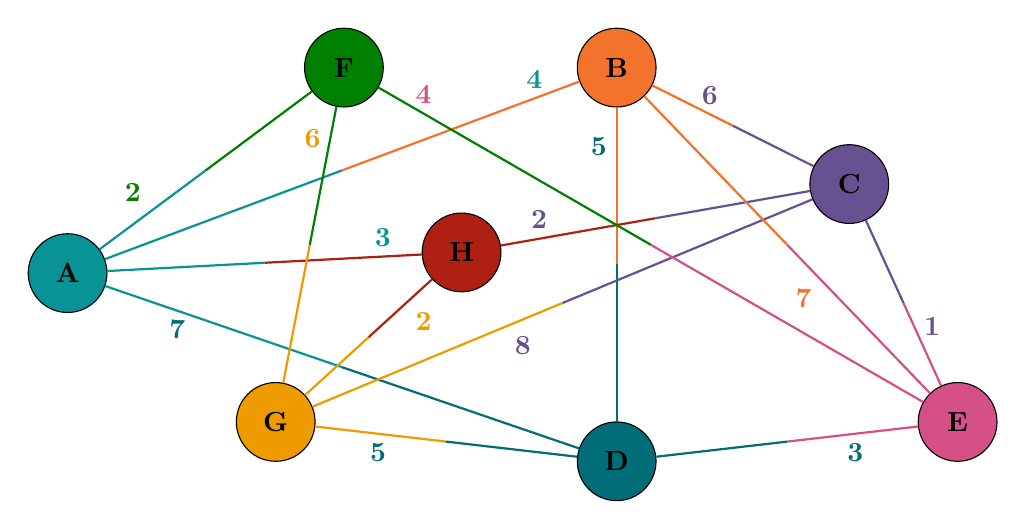
\begin{tikzpicture}[
                    main/.style = {
                        draw=black, circle, minimum size=10mm, inner sep=1pt, font=\bfseries
                    }
                ]
                    % Define colors for each node
                    \definecolor{colorA}{HTML}{0a9396}
                    \definecolor{colorB}{HTML}{f3722c}
                    \definecolor{colorC}{HTML}{665191}
                    \definecolor{colorD}{HTML}{006d77}
                    \definecolor{colorE}{HTML}{d45087}
                    \definecolor{colorF}{HTML}{008000}
                    \definecolor{colorG}{HTML}{ee9b00}
                    \definecolor{colorH}{HTML}{ae2012}
                    
                    % Nodes
                    \node[main, fill=colorA] (A) at (185:7) {A};
                    \node[main, fill=colorB] (B) at (90:2) {B};
                    \node[main, fill=colorC] (C) at (10:3) {C};
                    \node[main, fill=colorD] (D) at (270:3) {D};
                    \node[main, fill=colorE] (E) at (330:5) {E};
                    \node[main, fill=colorF] (F) at (150:4) {F};
                    \node[main, fill=colorG] (G) at (210:5) {G};
                    \node[main, fill=colorH] (H) at (190:2) {H};

                    % Aristas: Pintar cada mitad por el color de sus nodos
                    % El 0.5 a otro valor entre 0 y 1 para mover la etiqueta a lo largo de la arista.
                    % Macro para las aristas de doble color.
                    \def\halflink#1#2#3#4#5{
                        \draw[thick, decoration={markings, mark=at position 0.5 with {\arrow{}}}, postaction={decorate}] 
                            ([shift={(#5)}]#1) -- ([shift={(#5)}]#2);
                        \draw[thick, color=#3] 
                            ([shift={(#5)}]#1) -- ([shift={(#5)}]#1)!0.5!([shift={(#5)}]#2);
                        \draw[thick, color=#4] 
                            ([shift={(#5)}]#1)!0.5!([shift={(#5)}]#2) -- ([shift={(#5)}]#2);
                    }

                    % A-B
                    \draw[thick, color=colorA] (A) -- ($(A)!0.5!(B)$);
                    \draw[thick, color=colorB] ($(A)!0.5!(B)$) -- (B);
                    \node[above, color=colorA, font=\bfseries] at ($(A)!0.85!(B)$) {4};

                    % A-D
                    \draw[thick, color=colorA] (A) -- ($(A)!0.5!(D)$);
                    \draw[thick, color=colorD] ($(A)!0.5!(D)$) -- (D);
                    \node[below, color=colorD, font=\bfseries] at ($(A)!0.2!(D)$) {7};

                    % A-F
                    \draw[thick, color=colorA] (A) -- ($(A)!0.5!(F)$);
                    \draw[thick, color=colorF] ($(A)!0.5!(F)$) -- (F);
                    \node[above left, color=colorF, font=\bfseries] at ($(A)!0.3!(F)$) {2};

                    % A-H
                    \draw[thick, color=colorA] (A) -- ($(A)!0.5!(H)$);
                    \draw[thick, color=colorH] ($(A)!0.5!(H)$) -- (H);
                    \node[above, color=colorA, font=\bfseries] at ($(A)!0.8!(H)$) {3};

                    % B-C
                    \draw[thick, color=colorB] (B) -- ($(B)!0.5!(C)$);
                    \draw[thick, color=colorC] ($(B)!0.5!(C)$) -- (C);
                    \node[above, color=colorC, font=\bfseries] at ($(B)!0.4!(C)$) {6};

                    % B-D
                    \draw[thick, color=colorB] (B) -- ($(B)!0.5!(D)$);
                    \draw[thick, color=colorD] ($(B)!0.5!(D)$) -- (D);
                    \node[left, color=colorD, font=\bfseries] at ($(B)!0.2!(D)$) {5};

                    % C-E
                    \draw[thick, color=colorC] (C) -- ($(C)!0.5!(E)$);
                    \draw[thick, color=colorE] ($(C)!0.5!(E)$) -- (E);
                    \node[right, color=colorC, font=\bfseries] at ($(C)!0.6!(E)$) {1};

                    % C-G
                    \draw[thick, color=colorC] (C) -- ($(C)!0.5!(G)$);
                    \draw[thick, color=colorG] ($(C)!0.5!(G)$) -- (G);
                    \node[below right, color=colorC, font=\bfseries] at ($(C)!0.6!(G)$) {8};

                    % C-H
                    \draw[thick, color=colorC] (C) -- ($(C)!0.5!(H)$);
                    \draw[thick, color=colorH] ($(C)!0.5!(H)$) -- (H);
                    \node[above, color=colorC, font=\bfseries] at ($(C)!0.8!(H)$) {2};

                    % D-E
                    \draw[thick, color=colorD] (D) -- ($(D)!0.5!(E)$);
                    \draw[thick, color=colorE] ($(D)!0.5!(E)$) -- (E);
                    \node[below, color=colorD, font=\bfseries] at ($(D)!0.7!(E)$) {3};

                    % E-B
                    \draw[thick, color=colorE] (E) -- ($(E)!0.5!(B)$);
                    \draw[thick, color=colorB] ($(E)!0.5!(B)$) -- (B);
                    \node[below left, color=colorB, font=\bfseries] at ($(E)!0.4!(B)$) {7};

                    % E-F
                    \draw[thick, color=colorE] (E) -- ($(E)!0.5!(F)$);
                    \draw[thick, color=colorF] ($(E)!0.5!(F)$) -- (F);
                    \node[above, color=colorE, font=\bfseries] at ($(E)!0.87!(F)$) {4};

                    % G-D
                    \draw[thick, color=colorG] (G) -- ($(G)!0.5!(D)$);
                    \draw[thick, color=colorD] ($(G)!0.5!(D)$) -- (D);
                    \node[below, color=colorD, font=\bfseries] at ($(G)!0.3!(D)$) {5};

                    % G-F
                    \draw[thick, color=colorG] (G) -- ($(G)!0.5!(F)$);
                    \draw[thick, color=colorF] ($(G)!0.5!(F)$) -- (F);
                    \node[left, color=colorG, font=\bfseries] at ($(G)!0.8!(F)$) {6};

                    % G-H
                    \draw[thick, color=colorG] (G) -- ($(G)!0.5!(H)$);
                    \draw[thick, color=colorH] ($(G)!0.5!(H)$) -- (H);
                    \node[below right, color=colorG, font=\bfseries] at ($(G)!0.7!(H)$) {2};
                \end{tikzpicture}
            \end{center}
            \begin{enumerate}[label=\alph*)]
                \item Aplique el algoritmo de Kruskal para encontrar el árbol de expansión mínima del grafo. Indique el orden en que se agregan las aristas y dibuje el árbol resultante.
                \item Aplique el algoritmo de Dijkstra para encontrar el camino más corto desde el nodo A a todos los demás nodos. Indique el orden en que se visitan los nodos y las distancias mínimas encontradas. Muestre la tabla de distancias finales para cada nodo.
            \end{enumerate}
        \end{enumerate}
    \end{titlepage}

    \newpage
        \begin{center}
            \textbf{RESPUESTAS}
        \end{center}

        \begin{enumerate}
            % RESPUESTA 1
            \item Un árbol AVL es un tipo de árbol binario de búsqueda auto-balanceado en el que, para cada nodo, la diferencia de alturas entre sus subárboles izquierdo y derecho (llamada factor de balance) es a lo sumo 1, es decir:
            
            \begin{equation*}
                | \text{altura(subárbol izquierdo)} - \text{altura(subárbol derecho)} | \leq 1
            \end{equation*}

            Esta propiedad garantiza que las operaciones de inserción, eliminación y búsqueda tengan una complejidad temporal \(O(\log n)\), manteniendo el árbol balanceado mediante rotaciones cuando es necesario.

            % RESPUESTA 2
            \item La implementación del código la puede encontrar en la rama de ayudantías del repositorio del curso. \href{https://github.com/otrab/EDA/tree/ayudant%C3%ADas}{Link.}
            
            % RESPUESTA 3
            \item 
            \begin{enumerate}[label=\alph*)]
                \item Paso a paso de las inserciones y alturas:

                \begin{itemize}
                    \item \textbf{Insertar 50:}
                    \[
                        \begin{forest}
                            for tree={circle,draw,minimum size=1.2em,inner sep=1pt,s sep=3em,l=3em}
                            [50, label=above:1]
                        \end{forest}
                    \]
                    Altura de 50: 1. No hay rotación.

                    \vspace{1em}
                    \item \textbf{Insertar 30:}
                    \[
                        \begin{forest}
                            for tree={circle,draw,minimum size=1.2em,inner sep=1pt,s sep=3em,l=3em}
                            [50, label=2
                                [30, label=1, xshift=-2em]
                            ]
                        \end{forest}
                    \]
                    Alturas: 50 (2), 30 (1). No hay rotación.

                    \vspace{1em}
                    \item \textbf{Insertar 70:}
                    \[
                        \begin{forest}
                            for tree={circle,draw,minimum size=1.2em,inner sep=1pt,s sep=3em,l=3em}
                            [50, label=2
                                [30, label=1]
                                [70, label=1]
                            ]
                        \end{forest}
                    \]
                    Alturas: 50 (2), 30 (1), 70 (1). No hay rotación.

                    \vspace{1em}
                    \item \textbf{Insertar 20:}
                    \[
                        \begin{forest}
                            for tree={circle,draw,minimum size=1.2em,inner sep=1pt,s sep=3em,l=3em}
                            [50, label=3
                                [30, label=2
                                    [20, label=1, xshift=-2em]
                                ]
                                [70, label=1]
                            ]
                        \end{forest}
                    \]
                    Alturas: 50 (3), 30 (2), 20 (1), 70 (1). No hay rotación.

                    \vspace{1em}
                    \item \textbf{Insertar 40:}
                    \[
                        \begin{forest}
                            for tree={circle,draw,minimum size=1.2em,inner sep=1pt,s sep=3em,l=3em}
                            [50, label=3
                                [30, label=2
                                    [20, label=1]
                                    [40, label=1]
                                ]
                                [70, label=1]
                            ]
                        \end{forest}
                    \]
                    Alturas: 50 (3), 30 (2), 20 (1), 40 (1), 70 (1). No hay rotación.

                    \vspace{1em}
                    \item \textbf{Insertar 60:}
                    \[
                        \begin{forest}
                            for tree={circle,draw,minimum size=1.2em,inner sep=1pt,s sep=3em,l=3em}
                            [50, label=3
                                [30, label=2
                                    [20, label=1]
                                    [40, label=1]
                                ]
                                [70, label=2
                                    [60, label=1, xshift=-2em]
                                ]
                            ]
                        \end{forest}       \]
                    Alturas: 50 (3), 30 (2), 70 (2), 20 (1), 40 (1), 60 (1). No hay rotación.

                    \vspace{1em}
                    \item \textbf{Insertar 80:}
                    \[
                        \begin{forest}
                            for tree={circle,draw,minimum size=1.2em,inner sep=1pt,s sep=3em,l=3em}
                            [50, label=3
                                [30, label=2
                                    [20, label=1]
                                    [40, label=1]
                                ]
                                [70, label=2
                                    [60, label=1]
                                    [80, label=1]
                                ]
                            ]
                        \end{forest}
                    \]
                    Alturas: 50 (3), 30 (2), 70 (2), 20 (1), 40 (1), 60 (1), 80 (1). No hay rotación.

                    \vspace{1em}
                    \item \textbf{Insertar 10:}
                    \[
                        \begin{forest}
                            for tree={circle,draw,minimum size=1.2em,inner sep=1pt,s sep=3em,l=3em}
                            [50, label=4
                                [30, label=3
                                    [20, label=2
                                        [10, label=1, xshift=-2em]
                                ]
                                    [40, label=1]
                                ]
                                [70, label=2
                                    [60, label=1]
                                    [80, label=1]
                                ]
                            ]
                        \end{forest}
                    \]
                    Alturas: 50 (4), 30 (3), 70 (2), 20 (2), 40 (1), 60 (1), 80 (1), 10 (1). No hay rotación.

                    \vspace{1em}
                    \item \textbf{Insertar 5:}
                    \[
                        \begin{forest}
                            for tree={circle,draw,minimum size=1.2em,inner sep=1pt,s sep=3em,l=3em}
                            [50, label=5
                                [30, label=4
                                    [20, label=3
                                        [10, label=2, xshift=-2em
                                            [5, label=1, xshift=-4em]
                                        ]
                                    ]
                                    [40, label=1]
                                ]
                                [70, label=2
                                    [60, label=1]
                                    [80, label=1]
                                ]
                            ]
                        \end{forest}
                    \]
                    Alturas: 50 (5), 30 (4), 20 (3), 70 (2), 10 (2), 5 (1), 40 (1), 60 (1), 80 (1). \\
                    \textbf{Rotación:} Hay un desbalance en el nodo 30 (factor de balance = 3 en el subárbol izquierdo y 1 en el derecho), por lo que se realiza una \textbf{rotación simple a la derecha} en el nodo 20 para balancear el árbol. El árbol resultante es:

                    \[
                        \begin{forest}
                            for tree={circle,draw,minimum size=1.2em,inner sep=1pt,s sep=3em,l=3em}
                            [50, label=4
                                [30, label=3
                                    [10, label=2
                                        [5, label=1, xshift=-2em]
                                        [20, label=1, xshift=2em]
                                    ]
                                    [40, label=1]
                                ]
                                [70, label=2
                                    [60, label=1]
                                    [80, label=1]
                                ]
                            ]
                        \end{forest}
                    \]
                    Alturas: 50 (4), 30 (3), 10 (2), 70 (2), 5 (1), 20 (1), 40 (1), 60 (1), 80 (1).
                \end{itemize}

                \item \textbf{Rotaciones realizadas:}
                \begin{itemize}
                    \item Insertar 50: Ninguna rotación.
                    \item Insertar 30: Ninguna rotación.
                    \item Insertar 70: Ninguna rotación.
                    \item Insertar 20: Ninguna rotación.
                    \item Insertar 40: Ninguna rotación.
                    \item Insertar 60: Ninguna rotación.
                    \item Insertar 80: Ninguna rotación.
                    \item Insertar 10: Ninguna rotación.
                    \item Insertar 5: Rotación simple a la derecha con pivote en el nodo 20.
                \end{itemize}                
            \end{enumerate}

            \newpage
            % RESPUESTA 4
            \item
            \begin{enumerate}[label=\alph*)]
                \item \textbf{Kruskal:} Ordenamos las todas las aristas de menor a mayor peso.
                
                \begin{center}
                    \begin{tabular}{|c|c|}
                        \hline
                        \textbf{Arista} & \textbf{Peso} \\
                        \hline
                        C--E & 1 \\
                        \hline
                        A--F & 2 \\
                        \hline
                        C--H & 2 \\
                        \hline
                        G--H & 2 \\
                        \hline
                        A--H & 3 \\
                        \hline
                        D--E & 3 \\
                        \hline
                        A--B & 4 \\
                        \hline
                        E--F & 4 \\
                        \hline
                        B--D & 5 \\
                        \hline
                        G--D & 5 \\
                        \hline
                        G--F & 6 \\
                        \hline
                        B--C & 6 \\
                        \hline
                        B--E & 7 \\
                        \hline
                        A--D & 7 \\
                        \hline
                        C--G & 8 \\
                        \hline
                    \end{tabular}
                \end{center} 

                Seleccionamos las 7 aristas de menor peso sin formar ciclos:
                \begin{itemize}
                    \item C--E (1)
                    \item A--F (2)
                    \item C--H (2)
                    \item G--H (2)
                    \item A--H (3)
                    \item D--E (3)
                    \item A--B (4)
                \end{itemize}

                \textbf{Árbol resultante:}
                \[
                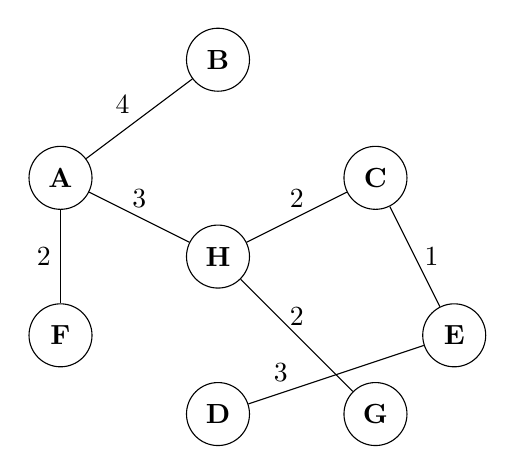
\begin{tikzpicture}[
                    main/.style = {draw=black, circle, minimum size=8mm, inner sep=1pt, font=\bfseries}
                ]
                    \node[main] (A) at (0,0) {A};
                    \node[main] (B) at (2,1.5) {B};
                    \node[main] (C) at (4,0) {C};
                    \node[main] (E) at (5,-2) {E};
                    \node[main] (F) at (0,-2) {F};
                    \node[main] (H) at (2,-1) {H};
                    \node[main] (G) at (4,-3) {G};
                    \node[main] (D) at (2,-3) {D};

                    \draw (A) -- node[left] {2} (F);
                    \draw (A) -- node[above] {3} (H);
                    \draw (A) -- node[left, yshift=0.5em] {4} (B);
                    \draw (C) -- node[right] {1} (E);
                    \draw (C) -- node[above] {2} (H);
                    \draw (G) -- node[above] {2} (H);
                    \draw (D) -- node[above, yshift=-0.6em, xshift=-2em] {3} (E);
                \end{tikzpicture}
                \]

                \item \textbf{Dijkstra (desde A):}

                Iniciamos las distancias \(d(A)=0\), \(d(\text{resto})=\infty\). Conjunto U vacío.

                \begin{enumerate}[label=\arabic*.]
                    \item Tomamos \textbf{A} (dist=0). Actualizamos:
                    \[d(B)=4,\ d(D)=7,\ d(F)=2,\ d(H)=3.\]
                    \item Tomamos el menor en \(V \notin     U\): \textbf{F} (2). Actualizamos: \(d(E)=2+4=6,\ d(G)=2+6=8.\)
                    \item Siguiente: \textbf{H} (3). Actualizamos:\(d(C)=3+2=5,\ d(G)=\min(8,3+2=5)=5.\)
                    \item Siguiente: \textbf{B} (4). Sus aristas no mejoran distancias.
                    \item Siguiente: \textbf{C} (5). Actualizamos: \(d(E)=\min(6,5+1=6)=6.\)
                    \item Siguiente: \textbf{G} (5). Actualiza \(d(D)=\min(7,5+5=10)=7.\)
                    \item Siguiente: \textbf{E} (6). Sus aristas no mejoran distancias.
                    \item \textbf{D} (7). Fin.
                \end{enumerate}

                \textbf{Orden de visita:} A, F, H, B, C, E, G, D

                \textbf{Tabla de distancias finales:}

                \begin{center}
                    \begin{tabular}{|c|c|}
                        \hline
                        \textbf{Nodo} & \textbf{Distancia desde A} \\
                        \hline
                        A & 0 \\
                        \hline
                        B & 4 \\
                        \hline
                        C & 5 \\
                        \hline
                        D & 7 \\
                        \hline
                        E & 6 \\
                        \hline
                        F & 2 \\
                        \hline
                        G & 5 \\
                        \hline
                        H & 3 \\
                        \hline
                    \end{tabular}
                \end{center}      
            \end{enumerate}
        \end{enumerate}
\end{document}